%%%%%%%%%%%%%%%%%%%%%%%%%%%%%%%%%%%%%
%%%%   Begin Document  %%%%%%%
%%%%%%%%%%%%%%%%%%%%%%%%%%%%%%%%%%%%%
\documentclass[12pt, letterpaper]{article}
\usepackage[vmargin=1in, hmargin=1in]{geometry}
\usepackage{amsmath}
\usepackage{graphicx}
\begin{document}


%%%%%%%%%%%%%%%%%%%%%%%%%%%%%%%%%%%%%
%%%%%%%%%%   Heading    %%%%%%%%%%%%%
%%%%%%%%%%%%%%%%%%%%%%%%%%%%%%%%%%%%%
\noindent{Kevin Sliker}

\noindent{\today}

\noindent{CS261 Data Structures: Assignment 7}
\vspace{0.2in}


%%%%%%%%%%%%%%%%%%%%%%%%%%%%%%%%%%%%%
%%%%%%%%   Title of Paper     %%%%%%%
%%%%%%%%%%%%%%%%%%%%%%%%%%%%%%%%%%%%%
\begin{center}
	\textbf{Hash Tables}
\end{center}
\vspace{0.1in}

%%%%%%%%%%%%%%%%%%%%%%%%%%%%%%%%%%%%%
%%%%   Main Content         %%%%%%%%%
%%%%%%%%%%%%%%%%%%%%%%%%%%%%%%%%%%%%%
\begin{enumerate}
	\item Amy cannot simply increase the table size to 7 because the modulo in her algorithm would not return unique values given the third letter in each persons name. Specifically, the names Amy and Andy, with third letter values 24 and 3, respectively, modulo 7 gives the same remainder of 3. 
	\item 
		\begin{enumerate}
			\item Each name passed through Amy's hash function before modding:
				\begin{align*} 
					Abel &- 4\\ 
					Abigail &- 8\\ 
					Abraham &- 17\\  
					Ada &- 0\\ 
					Adam &- 0\\ 
					Adrian &- 17\\ 
					Adrienne &- 17\\ 
					Agnes &- 13\\ 
					Albert &- 1\\ 
					Alex &- 4\\ 
					Alfred &- 5\\ 
					Alice &- 8.
				\end{align*}
			\item Elements found in each bucket after being hashed:
				\begin{align*}
					\text{Table Size} &== 6       &        \text{Table Size} &==13 \\
					table[0] &= 2		& 	table[0] &= 3    \\
					table[1] &= 2		& 	table[1] &= 1    \\
					table[2] &= 2		& 	table[2] &= 0    \\
					table[3] &= 0		& 	table[3] &= 0    \\
					table[4] &= 2		& 	table[4] &= 5    \\
					table[5] &= 4		& 	table[5] &= 1    \\
						&		&       table[6] &= 0	\\
						 &		&       table[7] &= 0	\\
						 &		&       table[8] &= 2	\\
						 &		&       table[9] &= 0	\\
						 &		&       table[10] &= 0	\\
						 &		&       table[11] &= 0	\\
						 &		&       table[12] &= 0	\\
				\end{align*}
			\item The load factors for a tablesize of 6 and 13, are 2 and .92, respectively.
		\end{enumerate}
	\item Using $cos(val)$ as a hash function over the integer values is a bad idea because the cosine function is sinusoidal. Therefore, the values -1 and 1 (both proper integer values) both return $\approx .999848$.
	\item 
		\begin{enumerate}
			\item Days of the week hash function with a table size of 10: Assign each letter of the word a value between 0-25, add up all of the letters values, divide that sum by the number of letters in the word, then mod that quotient by 10. This algorithm results in a near perfect hash with only 2 collisions.

			\item Months of the year hash function with a table size of 15:
		\end{enumerate}
	\item One way to search for a given value would be to keep the buckets in a dynamic array but make the links or chaining a balanced binary tree. The reason for using a tree instead of a linked list would be to quickly search through our chains. We know that if the load factor is set correctly we could achieve a best case $O(1)$ time complexity for finding keys. We also know that we can achieve a $O(log n)$ time complexity for a balanced binary tree. So I would suggest using an AVL tree instead of a linked list to do our chaining by either ranking the values in the tree based on their character values, time they were entered in the tree, or some other distinguishing factor. 
\end{enumerate}	

\newpage
\vspace{0.5in}
\begin{center}
	\textbf{Graphs}
\end{center}

\noindent{Construct a graph in which a depth first search will uncover a solution in fewer steps that will a breadth first search.}

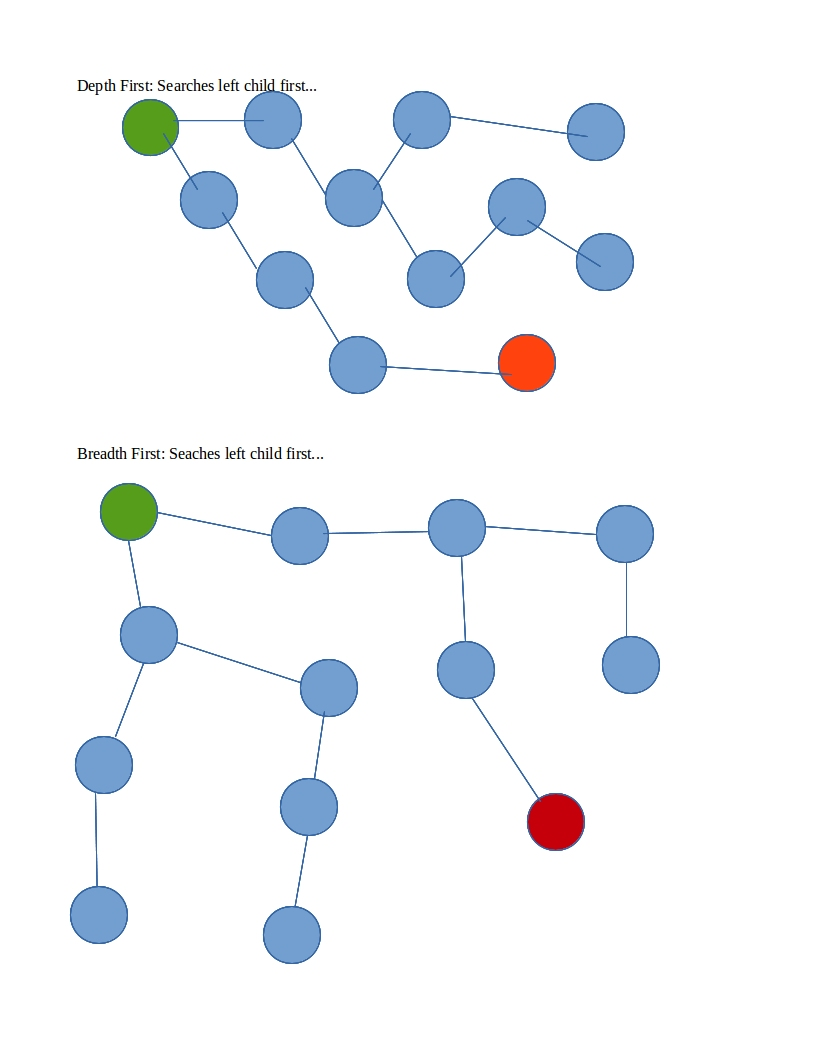
\includegraphics[scale=0.55]{graph}
\vspace{0.2in}

\newpage
\noindent{Complete worksheet 41}

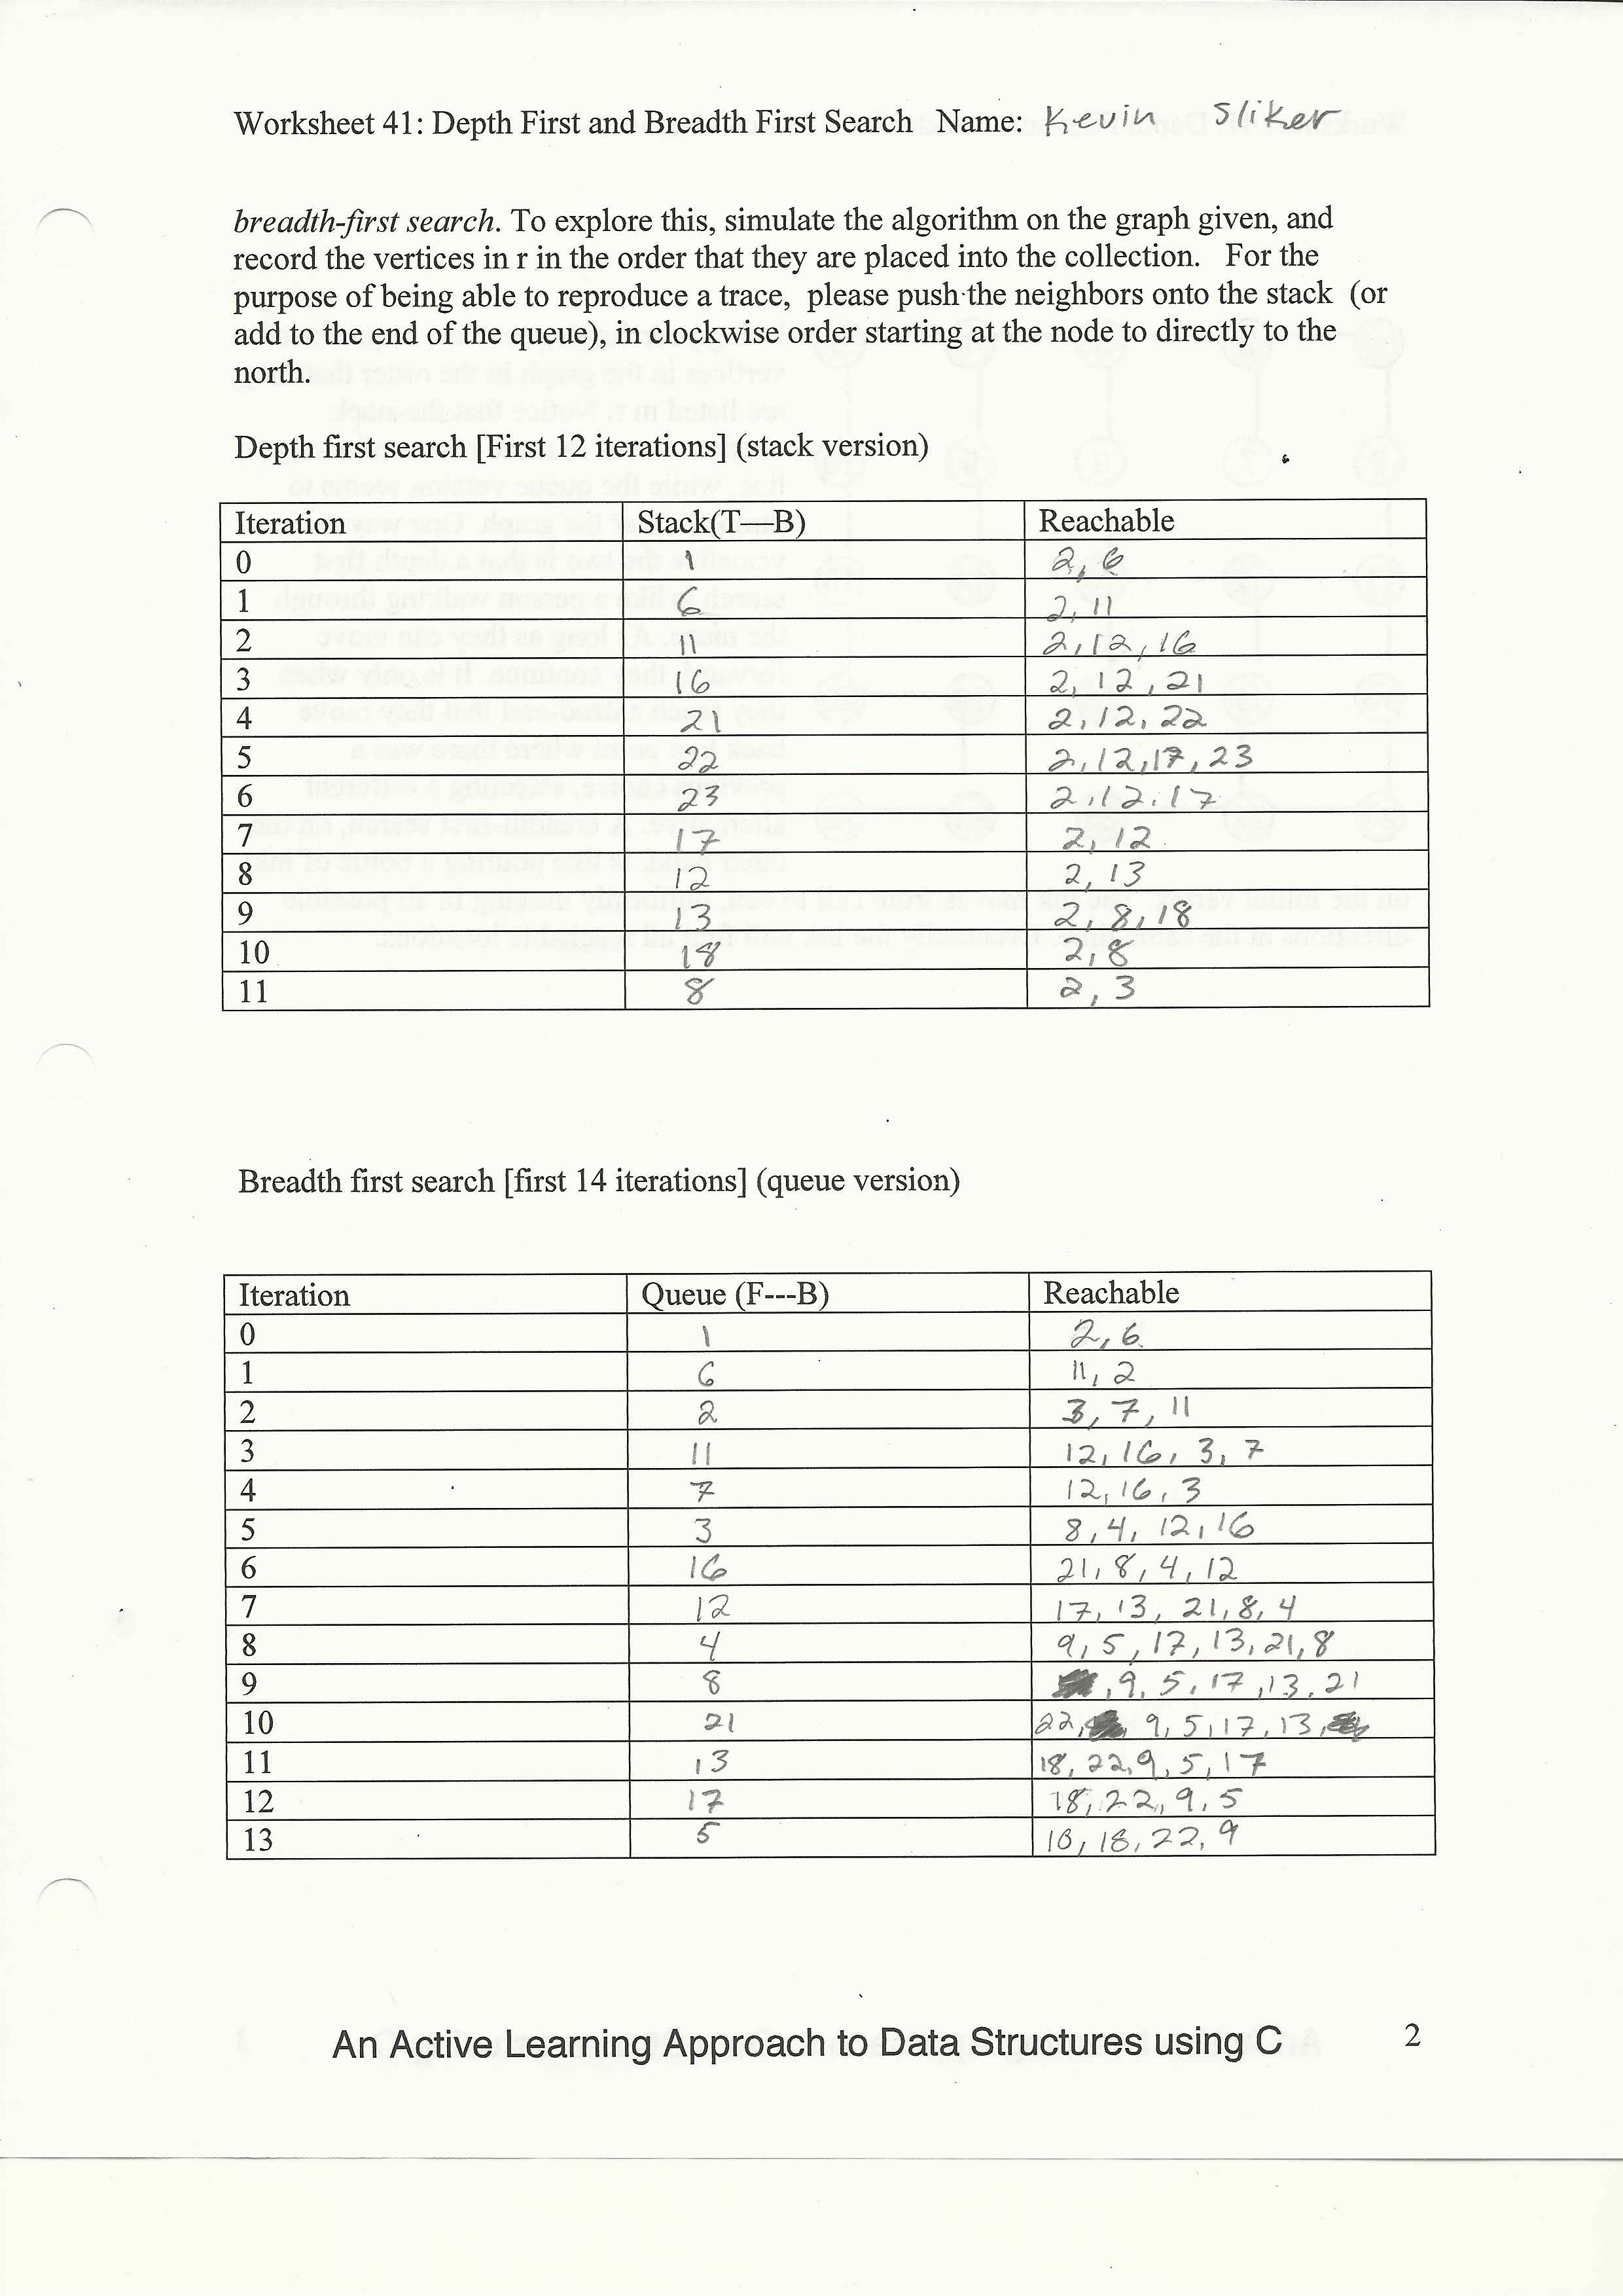
\includegraphics[scale=0.7]{41}


\newpage
\noindent{Complete worksheet 42}

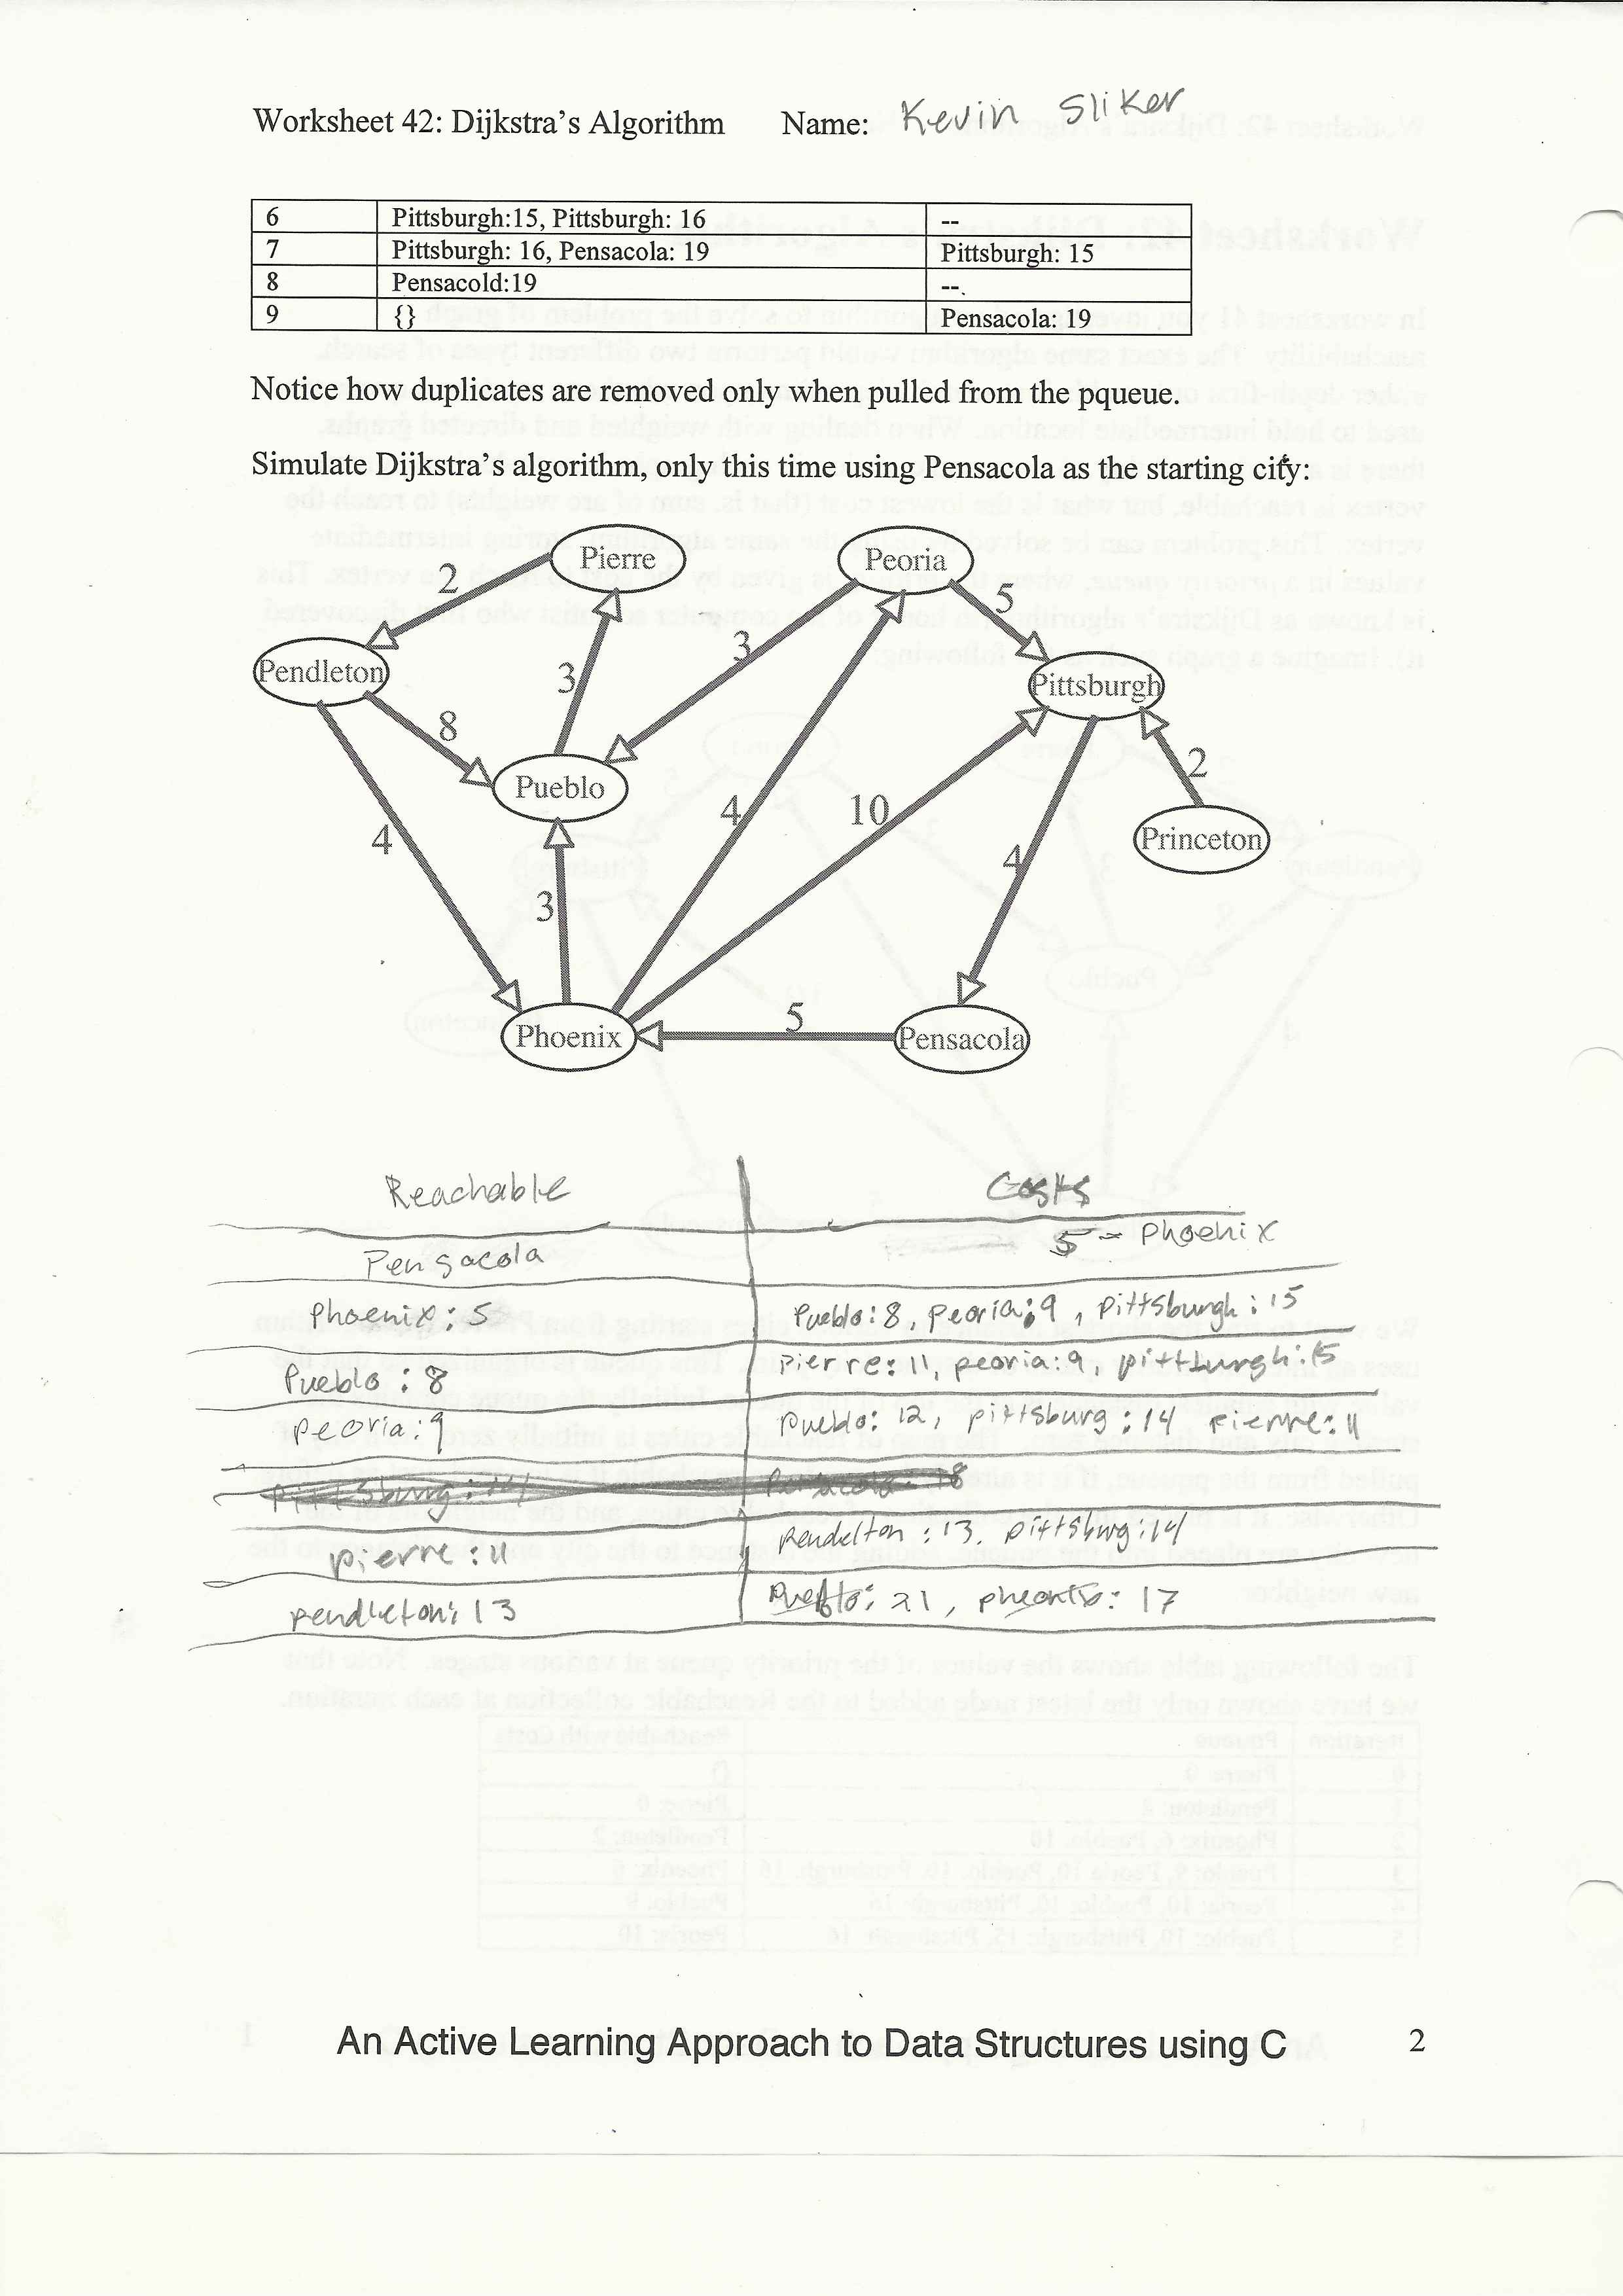
\includegraphics[scale=0.7]{42}


\newpage
\noindent\textbf{Why is it importatn that Dijkstra's algorithm stores intermediate results in a priority queue, rather than in an ordinary stack or queue?}

The importance in storing the intermediate results is that dijkstra's algorithm doesn't just want to find a path. It wants to find the path with the lowest cost. Therefore, when the algorithm is looking for potential paths it must hold the cost associated with each possible path in a priority to keep a preference. The algorithm is particular in which path it takes and the priority queue gives preference to those possible paths. The stack or the queue only give a ``backtracked" possible path, which is not necessarily a path of lowest cost.
\vspace{0.2in}

\noindent\textbf{How much space (in big-O notation) does an edge-list representation of a graph require?}

The edge-list would require $O(E)$ space for any number of edges - E.
\vspace{0.2in}

\noindent\textbf{For a graph with V vertices, how much space (in big-O notation) will an adjacency matrix require?}

The space for an adjacency matrix is $O(V^2)$ for any number of vertices - V.
\vspace{0.2in}

\noindent\textbf{Suppose you have a graph representing a maze that is infinite in size, but there is a finite path from the start to the finish. Is a depth first search guaranteed to find the path? Is a breadth-first search? Explain why or why not.}

The depth first search is not guaranteed to find the path to finish. The breadth first search is guaranteed to find a path to finish. The reason for this is due to the fact that if the depth first search chose a path that was infinite, it would never ``backtrack" to another path choice. That being said, it would carry out it's algorithm indefinitely. Now the depth first search would indeed find a path to finish even if there were an arbitrary amount of infinite paths as well. This method would search every possible path both the infinite ones and the finite ones all at the same time ensuring a completion in finite time.
%%%%%%%%%%%%%%%%%%%%%%%%%%%%%%%%%%%%%
%%%%%     End of Document    %%%%%%%%
%%%%%%%%%%%%%%%%%%%%%%%%%%%%%%%%%%%%%
\end{document}
